\section{Concepts}
\label{sec:concepts}
\subsection{Unsupervised and Supervised Learning}
\label{subsec:concepts-un-supervised-learning}
\begin{frame}{\insertsubsection}
    Supervised
    \pause
    \begin{itemize}[<+->]
        \item Fit model to labelled data (ie. with 'ground truth')
        \item Data is usually obtained experimentally or assigned by humans
        \item Previously labelled data can serve as testing set
    \end{itemize}
    \pause
    Unsupvervised
    \pause
    \begin{itemize}[<+->]
        \item Data does not contain any labels (only inputs)
        \item Find structure in data (clustering, grouping)
    \end{itemize}
    \pause
    Semi-supervised
    \pause
    \begin{itemize}[<+->]
        \item Combine partly labeled data with partly unlabeled data
        \item Can have huge performance benefits compared to unsupervised learning
    \end{itemize}
    This section follows~\cite{Greener2021}.
\end{frame}
%
%
\subsection{Terms}
\label{subsec:concepts-terms}
\begin{frame}{\insertsubsection}
    \pause
    \begin{itemize}[<+->]
        \item Classification: Assign datapoints discrete categories (eg. cancerous, non-cancerous). Algorithms are called 'classifiers'.
        \item[] If discrete categories are mutually exclusive, we call them 'classes', otherwise 'labels'.
        \item Regression: Output continuous values (eg. predict free energy of protein system).
        \item Classification problems can also be solved with regression and thresholds/binning.
        \item Clustering: Predict groupings of similar datapoints.
    \end{itemize}
\end{frame}
%
%
\begin{frame}{\insertsubsection}
    \begin{itemize}[<+->]
        \item Loss or Cost function:\\
        Measure deviation to ground truth in supervised learning.
        Implemented similarly in unsupervised situations.
        \item Parameters: Part of the model, will be adjusted by learning process of the model.
        \item Hyperparameters: Not part of the model but control learning process (eg. learning rate, number of iterations)
        \item Training: describes process of iterative learning and adjusting the parameters of the model to obtain better performance. Minimize the loss/cost-function.
        \item Validation: Use seperate dataset to test model.
    \end{itemize}
\end{frame}
%
%
\begin{frame}{\insertsubsection}
    \begin{figure}
        \centering
        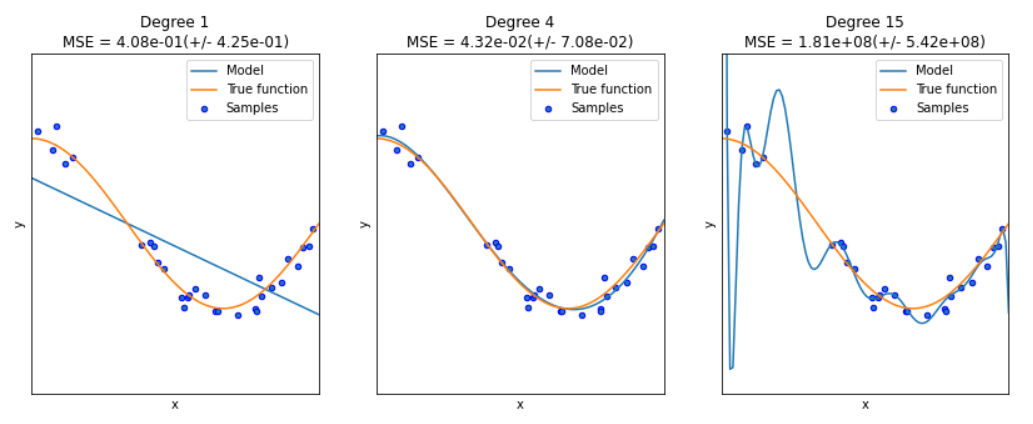
\includegraphics[width=\textwidth]{media/underfitting_and_overfitting_in_machine_learning_image.png}
        \caption{Underfitting, Optimal Fitting and Overfitting~\cite{Tripathi2020}}
    \end{figure}
\end{frame}
%
%
\subsection{Inductive Bias and Variance}
\label{subsec:concepts-bias-variance}
\begin{frame}{\insertsubsection}
    \begin{itemize}[<+->]
        \item Inductive Bias: Set of assumptions.
        \item[] Leads it to favour a particular type of solution over others.
        \item[] Often programmed in mathematical model.
        \item[] Example: Recurrent Neural Networks anticipate sequential dependencies
        \item Trade-off between bias and variance
        \item[] Different inductive biases typically lead to better performance, but higher constraints on the model.
        \item[] Lower bias makes fewer assumptions.
        \item Variance: How much does trained model change in response to training on different dataset.
        \item We want low bias and low variance.
        \item Low bias and low variance often conflict each other.
        \item[]$\Rightarrow$ Need to balance between them
    \end{itemize}
\end{frame}